\documentclass[sigconf,anonymous,review]{acmart}

\setcopyright{none}
\copyrightyear{2027}
\acmYear{2027}
\acmDOI{}
\acmConference[WSDM Submission]{ACM International Conference on Web Search and Data Mining}{Under review}{}
\acmISBN{}
\settopmatter{printacmref=true, printfolios=true}
\renewcommand\footnotetextcopyrightpermission[1]{}

\AtBeginDocument{%
  \providecommand\BibTeX{{Bib\TeX}}}
\newcommand{\sd}[1]{{\footnotesize$\pm$#1}}
\newcommand{\sigmark}[1]{\rlap{\textsuperscript{\scriptsize #1}}}
\usepackage{placeins}
\raggedbottom

\begin{document}

\title{Course-Knowledge Guided Reinforcement Learning for Strict Item-Cold MOOC Recommendation}

\begin{abstract}
MOOC platforms must recommend courses before interaction evidence has accumulated for them. This item-cold condition is often obscured by sampled ranking or interaction-weighted averages, where a method can perform well on frequent cold-course interactions while leaving other cold courses effectively unrecommended. We study strict item-cold MOOC recommendation: test cold courses have zero training interactions, compete against the full catalog, and are evaluated by item-macro Recall and NDCG. We propose Course-Knowledge Guided Reinforcement Learning (CKG-RL), which combines content-anchored course representations, forced-cold ID masking, retrieval-based user simulation, and educational rewards derived from concepts, prerequisites, difficulty, and redundancy. In three-seed evaluations, CKG-RL improves MOOCCube Recall@10 and NDCG@10 over CGRC from 0.2589/0.1845 to 0.2667/0.1962. The Junyi evaluation gives the same primary cold-side ordering, and on COCO CKG-RL improves Recall@10 and NDCG@10 from 0.0656/0.0332 for CCFCRec to 0.0679/0.0392. Ablations show that educational rewards, knowledge-guided sampling, and prerequisite supervision each contribute under the strict item-cold evaluator. The results support a protocol-aware view of cold-start recommendation: reducing item-cold exposure risk requires both content transfer and educational constraints.
\end{abstract}

\begin{CCSXML}
<ccs2012>
   <concept>
       <concept_desc>Information systems~Recommender systems</concept_desc>
       <concept_significance>500</concept_significance>
   </concept>
   <concept>
       <concept_desc>Applied computing~Interactive learning environments</concept_desc>
       <concept_significance>300</concept_significance>
   </concept>
</ccs2012>
\end{CCSXML}

\ccsdesc[500]{Information systems~Recommender systems}
\ccsdesc[300]{Applied computing~Interactive learning environments}

\keywords{MOOC recommendation, item cold-start, reinforcement learning, educational data mining, course knowledge}

\maketitle

\section{Introduction}
MOOC platforms continuously add new courses, course versions, and learning paths. Their recommender systems must therefore do more than match learners with familiar popular courses. They must also give newly introduced or rarely observed courses a plausible route to suitable learners before those courses have accumulated interaction evidence. This item-side cold-start condition is especially consequential in education, where a suitable course depends on topical relevance, prerequisite readiness, difficulty, and redundancy with prior learning.

Standard offline evaluation can hide this condition. Sampled candidate sets may remove the warm courses that dominate the full catalog, and interaction-weighted averages may be driven by a few cold courses with many test interactions. Under either choice, a model can obtain a competitive average score while leaving some item-cold courses effectively unrecommended. This is a course-level exposure risk: the average interaction may be served well, while a tail set of courses receives no useful exposure. Recent risk-sensitive ranking work makes an analogous point for search diversification, where optimizing average utility can leave minority intents poorly served~\cite{takehi2025diversification}. We adopt this evaluation logic for item-cold course recommendation.

This paper studies \emph{strict item-cold MOOC recommendation}. Cold test courses have zero interactions in the training set, and they are evaluated against the full course catalog rather than sampled negatives. Our primary metric is item-macro Recall/NDCG: we first compute ranking utility for each held-out cold course and then average across courses. The metric therefore asks whether a randomly selected cold course is served well, not only whether a randomly selected cold-course interaction is served well.

The protocol implies two modeling requirements. First, a cold course must be represented without relying on interaction-trained ID evidence. Course text, concepts, prerequisites, and other side information are therefore the primary evidence for the target item rather than auxiliary features. Second, semantic similarity is not sufficient for educational recommendation. A course can be topically related to a learner while being too advanced, prerequisite-unsafe, or redundant. A strict item-cold model must transfer information from warm courses to cold courses while respecting these educational constraints.

We propose Course-Knowledge Guided Reinforcement Learning (CKG-RL), a framework designed around these requirements. CKG-RL uses content-anchored course representations and forced-cold ID masking to respect the evidence boundary of item-cold evaluation. It then runs a retrieval-based user simulation in which a policy updates the course state through plausible learner matches. Concept, prerequisite, difficulty, and redundancy signals shape both candidate construction and reward design, so course knowledge affects the ranking process rather than being appended only as static features.

The MOOCCube, Junyi, and COCO evaluations show that CKG-RL improves the primary strict item-cold full-ranking item-macro metrics. On MOOCCube, its R@10/N@10 is 0.2667/0.1962, compared with 0.2589/0.1845 for CGRC. On Junyi, it gives consistent cold-item gains over the corrected CGRC baseline. On COCO, its R@10/N@10 is 0.0679/0.0392, compared with 0.0656/0.0332 for CCFCRec. The evidence is organized around one question: whether a method reduces item-cold exposure risk under full-catalog competition.

The contributions are as follows:
\begin{itemize}
    \item We formulate item-cold MOOC recommendation as a strict item-heldout ranking problem and use full-ranking item-macro metrics as the primary evaluation target.
    \item We introduce CKG-RL, a course-knowledge guided reinforcement learning framework that combines content anchoring, forced-cold handling, and educational rewards.
    \item We conduct three-seed experiments on MOOCCube, Junyi, and COCO against collaborative, graph, content-based, and cold-start baselines.
    \item We provide ablation evidence showing that concept, prerequisite, difficulty, and redundancy signals affect item-cold ranking under the same full-ranking protocol.
\end{itemize}

\section{Related Work}
\subsection{MOOC and Educational Recommendation}
Educational recommendation differs from general item recommendation because items carry pedagogical structure. MOOC datasets such as MOOCCube and MOOCCubeX provide interactions, course metadata, concepts, teachers, schools, and prerequisite relations for studying this structure~\cite{yu2020mooccube,wang2021mooccubex}. Existing MOOC recommenders have used sequential decision models and explainable path reasoning to connect learners with courses~\cite{zhang2019hrlcourse,dessi2024findingpaths}. A useful course recommendation should match learner interest while also considering knowledge readiness and learning path coherence. In this paper, concepts, prerequisite edges, difficulty proxies, and redundancy proxies are used as course-side evidence that remains available before the target course has interactions.

\subsection{Cold-Start Recommendation}
Cold-start recommendation addresses insufficient interaction history. Classical work studies how side attributes can be mapped into collaborative latent spaces for users or items with few observations~\cite{schein2002coldstart,gantner2010attribute}. A recent survey organizes cold-start evidence around content features, graph relations, domain knowledge, and emerging large-language-model-based signals~\cite{zhang2025coldstartllm}. Collaborative filtering methods such as BPR~\cite{rendle2009bpr} and graph-based recommenders~\cite{wang2019neuralgraphcollaborativefiltering,he2020lightgcn,ying2018graphconvolutional} are effective when enough interactions exist, but item cold-start requires the model to rank items whose IDs provide little or no supervised signal.

Recent item-cold methods include dropout-based training~\cite{volkovs2017dropoutnet}, contrastive view alignment~\cite{zhou2023ccfcrec}, aligned distillation~\cite{huang2023aldi}, content-based graph reconstruction~\cite{kim2024cgrc}, out-of-vocabulary item refinement~\cite{zhao2024usim}, feature-structure completion~\cite{zhao2025fsgnn}, popularity-aware meta-learning for online item cold-start~\cite{luo2025pam}, and item-centric exploration~\cite{jiang2025itemcentric}. These approaches transfer information from warm items to cold items through side information, meta-learning, graph completion, or controlled exploration. Our setting keeps this transfer problem but adds two constraints: cold courses compete against the full catalog, and educational relations should guide which learner-course matches are plausible.

\subsection{Risk-Sensitive Ranking Evaluation}
Offline recommender evaluation is sensitive to candidate construction and averaging choices. Sampled negative evaluation can change method comparisons relative to full-ranking evaluation~\cite{krichene2020sampled}, and reproducibility studies have shown that recommender gains can be fragile when baselines and validation protocols are not carefully controlled~\cite{dacrema2019progress}. Recent ranking work frames diversification as risk minimization: a system should not only improve average utility but also reduce failures on poorly served intents or tail cases~\cite{takehi2025diversification}. We adapt this lens to item-cold course recommendation. The tail unit is not an intent but a held-out cold course, and the risk is that the course receives no useful exposure under full-catalog ranking.

\subsection{Reinforcement Learning for Recommendation}
Reinforcement-learning-based recommenders model recommendation as sequential decision making~\cite{shani2005mdp,zhao2018deepreinforcement,chen2023rlrecsurvey}. This perspective is useful for education because recommendations may affect future learning trajectories. CKG-RL uses this idea in a narrower way: the simulator is a training mechanism for exploring learner-course matches under item-cold evidence constraints. The policy is guided by course knowledge and optimized jointly with ranking losses, with the final claim evaluated by strict item-cold full-ranking metrics.

\section{Problem Formulation}

\subsection{Preliminaries}
Let \(\mathcal{U}\) denote the set of learners and \(\mathcal{I}\) denote the set of courses. Each observed interaction is represented as \((u,i,t)\), where learner \(u \in \mathcal{U}\) interacted with course \(i \in \mathcal{I}\) at time \(t\). Given the training interactions \(\mathcal{D}_{\mathrm{train}}\) and course-side information, a recommender produces, for each learner \(u\), a ranked list \(\pi_u\) over candidate courses.

Each course \(i\) is associated with a content vector \(\mathbf{x}_i\) and a set of educational signals. We use concept overlap to model topical continuity, prerequisite links to approximate readiness, training popularity as a weak difficulty proxy, and similarity to the learner history as a redundancy proxy. These signals are not assumed to be complete measurements of learning state. They are course-side evidence that remains available even when the course has no training interactions.

\subsection{Strict Item-Cold Protocol}
We study an item-heldout cold-start setting. The course set is partitioned into warm courses \(\mathcal{I}_{\mathrm{warm}}\) and cold test courses \(\mathcal{I}_{\mathrm{cold}}\). A course \(i \in \mathcal{I}_{\mathrm{cold}}\) satisfies
\begin{equation}
|\{(u,j,t)\in \mathcal{D}_{\mathrm{train}}: j=i\}|=0.
\end{equation}
Thus, the model cannot rely on interaction-trained evidence for the target course ID. Its representation must be inferred from course content and educational knowledge.

For a test pair \((u,i^+)\) with \(i^+\in\mathcal{I}_{\mathrm{cold}}\), the candidate set is the full catalog after removing courses already observed in the learner's training history:
\begin{equation}
\mathcal{C}_u=\mathcal{I}\setminus \mathcal{H}^{\mathrm{train}}_u .
\end{equation}
The model scores all courses in \(\mathcal{C}_u\), so an item-cold course must compete directly with warm courses that have richer interaction evidence. The split is item-based rather than user-based: learners in cold-course test cases have training histories, while the target courses have none. This protocol isolates item-cold generalization under full-catalog competition.

\subsection{Standard Interaction Average}
Let \(m_K(u,i^+)\) denote a top-\(K\) utility for a test pair, instantiated as Recall@\(K\) or NDCG@\(K\). Let \(r_{u,i^+}\) be the rank of target course \(i^+\) in \(\pi_u\). Recall@\(K\) equals one when \(r_{u,i^+}\le K\) and zero otherwise, and NDCG@\(K\) is
\begin{equation}
\operatorname{NDCG@K}(u,i^+)=
\begin{cases}
1/\log_2(r_{u,i^+}+1), & r_{u,i^+}\le K,\\
0, & r_{u,i^+}>K.
\end{cases}
\end{equation}
Since each test case contains one held-out positive course, these metrics measure whether the target cold course is surfaced early enough in the full ranking.

A common evaluation choice is to average the utility over cold-course test interactions:
\begin{equation}
M_{\mathrm{micro}}(K)=
\frac{1}{|\mathcal{D}^{\mathrm{cold}}_{\mathrm{test}}|}
\sum_{(u,i^+)\in \mathcal{D}^{\mathrm{cold}}_{\mathrm{test}}}
m_K(u,i^+).
\end{equation}
This metric answers whether a randomly sampled cold-course interaction is ranked well. It is useful for measuring interaction-level utility, but it does not directly measure whether each cold course receives adequate exposure.

\subsection{Cold-Course Risk Metric}
Strict item-cold recommendation has a course-level failure mode: a model can serve high-volume cold courses while leaving other cold courses effectively unrecommended. To expose this risk, we aggregate first within each cold course. For course \(i\), let
\begin{equation}
q_i(K)=
\frac{1}{|\mathcal{D}_{\mathrm{test}}(i)|}
\sum_{(u,i)\in \mathcal{D}_{\mathrm{test}}(i)}
m_K(u,i),
\end{equation}
where \(\mathcal{D}_{\mathrm{test}}(i)\) is the set of test cases whose target course is \(i\). The item-macro metric is then
\begin{equation}
M_{\mathrm{macro}}(K)=
\frac{1}{|\mathcal{I}_{\mathrm{cold}}|}
\sum_{i\in\mathcal{I}_{\mathrm{cold}}} q_i(K).
\end{equation}
Interaction-micro and item-macro metrics therefore answer different questions: micro averaging asks whether a random cold-course interaction is served well, whereas item-macro averaging asks whether a random cold course is served well. We use the latter as the primary metric because the target risk in this paper is the failure to surface particular item-cold courses under full-catalog ranking.

This aggregation can reverse the preferred model when cold-course interaction counts are imbalanced. A high-volume model may obtain a stronger interaction average by serving a frequent cold course while completely missing a low-volume cold course. A broader-coverage model can have a lower interaction average but a higher course-level score. This is the cold-course analogue of a tail-risk failure: average interaction utility can improve while an individual cold course receives no useful exposure.

\subsection{Main Objective}
The objective of this paper is to improve full-ranking item-macro performance for courses with zero training interactions. Formally, the model should learn a scoring function \(s(u,i)\) that ranks \(i^+\in\mathcal{I}_{\mathrm{cold}}\) highly within \(\mathcal{C}_u\), using learner history and course-side evidence but no interaction-derived target-course signal. The protocol is a strict item-heldout benchmark for item-cold generalization. Hot-course metrics are reported as diagnostics of the trade-off between cold-course performance and warm-course ranking behavior.

\section{Method}
\subsection{Overview}
CKG-RL is designed to make the evidence boundary of strict item-cold ranking explicit. For each learner-course pair \((u,i)\), the model builds a learner representation \(\mathbf{z}_u\) from the learner history and a course representation \(\mathbf{q}_i\) from course-side evidence. A simulator then starts from \(\mathbf{q}_i\), refines it through \(T\) imagined user-matching steps, and returns a final state \(\mathbf{h}_T\). The ranking score is computed by matching \(\mathbf{h}_T\) with the target learner representation.

The framework follows three design constraints. First, a cold course cannot be represented by an interaction-trained ID shortcut, so the representation must be anchored in content. Second, full-catalog ranking makes cold courses compete with warm courses that have stronger collaborative evidence, so training should expose cold-course representations to plausible learner states rather than only to static content similarity. Third, educational relevance is constrained: a course may be semantically related but prerequisite-unsafe, too difficult, or redundant. CKG-RL maps these constraints to representation, masking, simulation, and reward design. Figure~\ref{fig:ckg-rl-framework} summarizes the resulting training and evaluation flow.

\begin{figure*}[t]
\centering
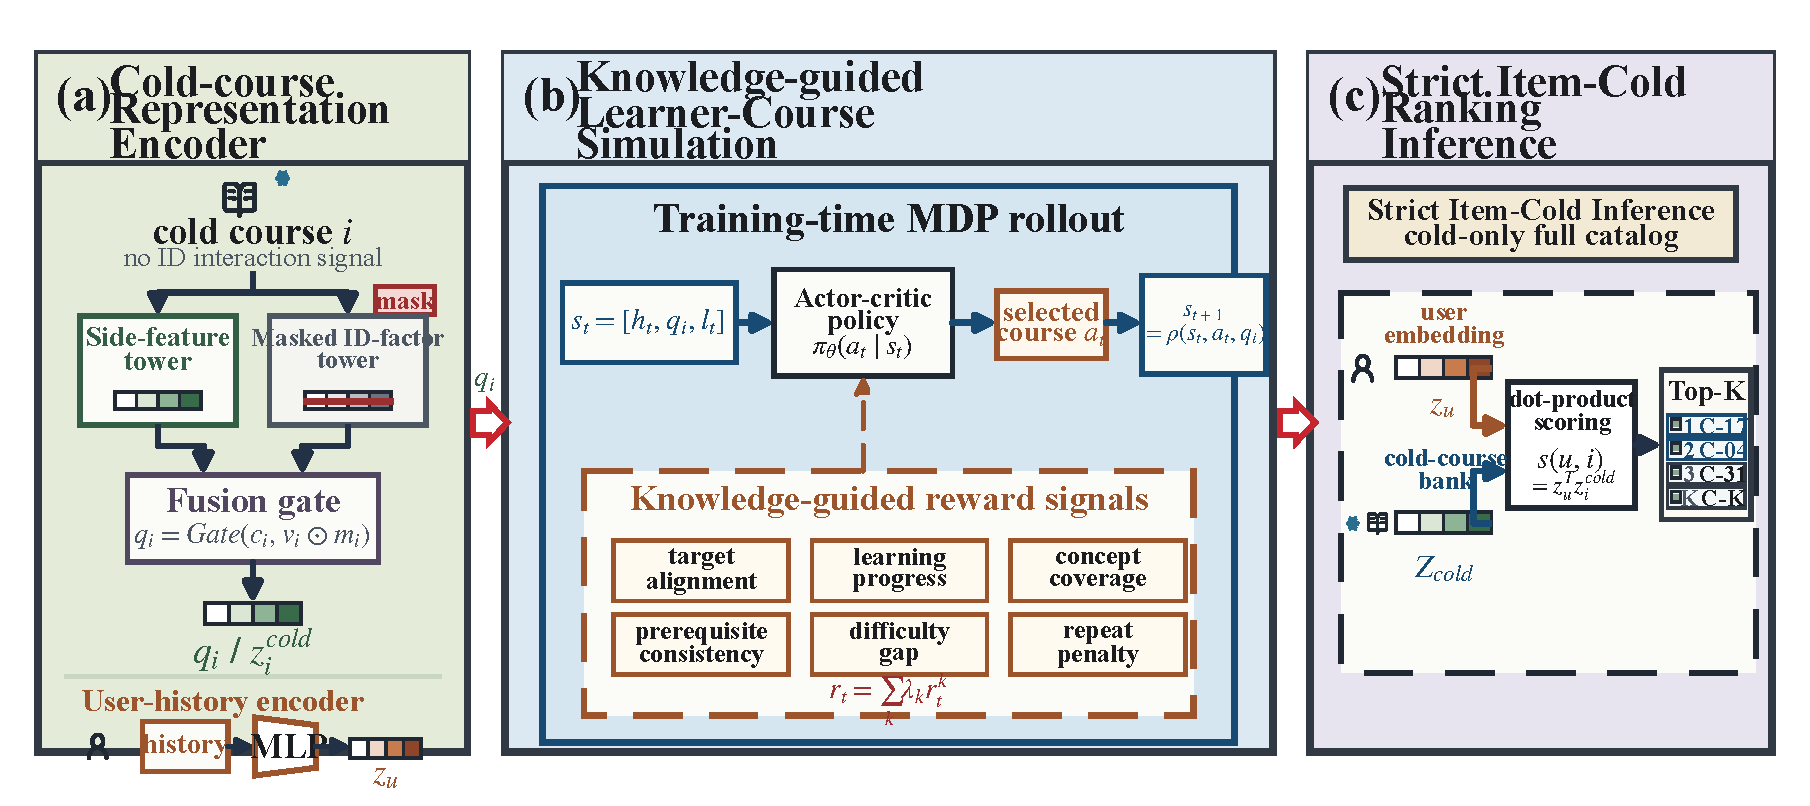
\includegraphics[width=0.98\textwidth]{figures/ckg_rl_framework_topconf.pdf}
\caption{CKG-RL pipeline for strict item-cold MOOC recommendation. The model masks target-course ID evidence for cold items, initializes the simulator from content-anchored course representations, refines the course state through knowledge-guided learner retrieval, and ranks cold courses against the full catalog with item-macro Recall/NDCG as the primary target.}
\Description{A three-panel framework diagram. The left panel shows course-side evidence and forced-cold ID masking. The middle panel shows a learner-course simulator with actor-critic selection, course-fit sampling, and course-knowledge reward feedback. The right panel shows strict item-cold full-catalog ranking and the optimization losses.}
\label{fig:ckg-rl-framework}
\end{figure*}

\subsection{Content-Anchored Course Representation}
The content branch provides the evidence that remains available for a course with zero training interactions. Each learner \(u\) has a trainable ID embedding \(\mathbf{e}_u\), projected into the recommendation space:
\begin{equation}
\mathbf{z}_u=f_u(\mathbf{e}_u).
\end{equation}
Each course \(i\) has a trainable ID embedding \(\mathbf{v}_i\) and a frozen 768-dimensional content embedding \(\mathbf{x}_i\). A content projection network maps \(\mathbf{x}_i\) into the same latent space:
\begin{equation}
\mathbf{c}_i=f_c(\mathbf{x}_i).
\end{equation}
The final course representation is a gated fusion of the projected content vector and a possibly masked ID vector:
\begin{equation}
\mathbf{g}_i=\sigma\left(\mathbf{W}_g[\bar{\mathbf{v}}_i;\mathbf{c}_i]\right),
\quad
\mathbf{q}_i=\mathbf{g}_i\odot \bar{\mathbf{v}}_i+(1-\mathbf{g}_i)\odot \mathbf{c}_i.
\end{equation}
Here \(\bar{\mathbf{v}}_i\) is the ID branch after masking and ID dropout. The gate lets warm courses use collaborative evidence when available, while still allowing the content branch to define the representation when the ID branch is removed.

\subsection{Forced-Cold ID Masking}
Forced-cold masking operationalizes the protocol inside the model. Let \(p_i\) be the training-set popularity of course \(i\). Under the final strict item-cold protocol, a course is cold when \(p_i<1\), which is equivalent to having zero training interactions. For cold examples, CKG-RL removes the course ID evidence:
\begin{equation}
\bar{\mathbf{v}}_i=(1-\xi_i)\mathbf{v}_i,
\quad
\xi_i=\mathbb{I}[p_i<1].
\end{equation}
During training, ordinary ID dropout is additionally applied with probability \(0.35\). At cold-course evaluation time, the target course vector is also built with the ID branch masked. This keeps the representation used at inference aligned with the evidence available in the strict item-cold protocol.

\subsection{Retrieval-Based User Simulation}
Full-catalog item-cold ranking requires a course representation that can compete for plausible learners, not only a pointwise content score. The simulator therefore treats the course state as an object to be refined through retrieved learner evidence. It initializes \(\mathbf{h}_0=\mathbf{q}_i\). At step \(t\), it retrieves candidate learners from a normalized user bank by cosine similarity to \(\mathbf{h}_t\). Let \(\mathcal{N}_M(\mathbf{h}_t)\) be the top-\(M\) retrieved learners. CKG-RL samples \(N\) candidates from this set with a temperature-smoothed distribution and an exploration floor:
\begin{equation}
p(u'\mid \mathbf{h}_t)=
(1-\epsilon)\operatorname{softmax}
\left(\frac{\mathbf{h}_t^\top\mathbf{z}_{u'}}{\tau_s}\right)
+\frac{\epsilon}{M}.
\end{equation}
The sampled candidates are then reordered by a course-fit score:
\begin{equation}
b(u',i)=
w_c C(u',i)-w_p P(u',i)-w_d D(u',i)-w_r R(u',i),
\end{equation}
\begin{equation}
s_{sample}(u',i)=
\cos(\mathbf{h}_t,\mathbf{z}_{u'})
+\beta\operatorname{norm}(b(u',i)).
\end{equation}
The four terms \(C\), \(P\), \(D\), and \(R\) are the concept bonus, prerequisite gap, difficulty gap, and redundancy penalty defined below. This knowledge-guided sampling bias is applied to both cold and hot examples in the final run, so retrieved candidates are filtered not only by latent similarity but also by educational plausibility.

An actor-critic policy selects a learner \(a_t\) from the sampled candidates. CKG-RL then updates the course state by taking a gradient step toward a mixture of the selected learner and the target course representation:
\begin{equation}
\mathbf{h}_{t+1}=\mathbf{h}_t+\eta
\nabla_{\mathbf{h}_t}
\left[
(1-\alpha_t)\mathbf{h}_t^\top\mathbf{z}_{a_t}
+\alpha_t\mathbf{h}_t^\top\mathbf{q}_i
\right].
\end{equation}
The target coefficient is adaptive:
\begin{align}
\alpha_t=
\operatorname{clip}_{[\alpha_{\min},\alpha_{\max}]}\Big(
&\alpha_{cold}\xi_i+\alpha_{hot}(1-\xi_i) \nonumber\\
&+\alpha_{step}\frac{t}{T-1}
-\alpha_{ent}\frac{H(\pi_t)}{\log N}
\Big).
\end{align}
Thus cold courses receive stronger target anchoring, later updates within the simulator horizon increase target guidance, and high-entropy actions reduce overconfident target drift. The simulation is not used to claim a real learner trajectory; it is a training-time mechanism for making the cold-course representation stable under plausible learner matches.

\subsection{Course-Knowledge Reward Design}
The reward terms convert educational constraints into training signals for the simulator. Let \(\mathbf{s}_u\in\{0,1\}^{|\mathcal{I}|}\) represent courses already seen by learner \(u\), and let \(n_u=\sum_j s_{u,j}\). Let \(\mathbf{A}^{pre}\) be the item-level prerequisite matrix derived from the MOOCCubeX concept prerequisite graph, and let \(\mathbf{A}^{con}\) be the item-concept overlap matrix. The signals below are proxy constraints rather than direct measurements of mastery, but they are available before the target course has interactions.

\paragraph{Prerequisite gap.}
The prerequisite gap estimates the fraction of required prerequisite evidence not covered by the learner history:
\begin{equation}
P(u,i)=
\left[
1-\frac{\mathbf{s}_u^\top \mathbf{A}^{pre}_{i}}
{\max(1,\|\mathbf{A}^{pre}_{i}\|_1)}
\right]_0^1.
\end{equation}
A prerequisite-safe gate \(S_{pre}(u,i)\) is one when the raw prerequisite gap is below the configured safety threshold and zero otherwise.

\paragraph{Concept bonus.}
The concept match between learner history and course concepts is
\begin{equation}
M(u,i)=
\left[
\frac{\mathbf{s}_u^\top \mathbf{A}^{con}_{i}}{\max(1,n_u)}
\right]_0^1.
\end{equation}
CKG-RL turns this match into a bounded concept bonus:
\begin{equation}
C(u,i)=
\left[
\frac{M(u,i)-\mu_c}{\mu_r-\mu_c}
\right]_0^1
\cdot S_{pre}(u,i)\cdot (1-\gamma_r R(u,i)).
\end{equation}

\paragraph{Difficulty gap.}
Course difficulty is estimated from inverse training popularity:
\begin{equation}
d_i=1-\frac{\log(1+p_i)}
{\max_j \log(1+p_j)}.
\end{equation}
Learner readiness is \(r_u=[n_u/n_{warm}]_0^1\), and the difficulty gap is
\begin{equation}
D(u,i)=\max(0,d_i-r_u).
\end{equation}

\paragraph{Redundancy penalty.}
When concept overlap is already high, the course may duplicate the learner's previous exposure. CKG-RL uses
\begin{equation}
R(u,i)=
\left[
\frac{M(u,i)-\mu_r}{1-\mu_r}
\right]_0^1.
\end{equation}

The step reward combines target preservation, progress toward the target representation, duplicate-action control, and the four course-knowledge terms:
\begin{align}
r_t=&-w_T\|\mathbf{h}_{t+1}-\mathbf{q}_i\|_2^2
+w_G\operatorname{clip}\left(
\|\mathbf{h}_t-\mathbf{q}_i\|_2^2
-\|\mathbf{h}_{t+1}-\mathbf{q}_i\|_2^2
\right) \nonumber\\
&-w_{dup}\operatorname{Dup}_t
+w_c C(a_t,i)-w_p P(a_t,i) \nonumber\\
&-w_d D(a_t,i)-w_r R(a_t,i).
\end{align}

\subsection{Optimization}
Optimization combines policy learning with ranking supervision. The actor-critic policy is optimized with PPO and generalized advantage estimation~\cite{schulman2017ppo,schulman2015gae}:
\begin{equation}
\delta_t=r_t+\gamma V(\mathbf{s}_{t+1})-V(\mathbf{s}_t),
\quad
\hat{A}_t=\sum_{l\geq 0}(\gamma\lambda)^l\delta_{t+l}.
\end{equation}
With probability ratio \(\rho_t(\theta)\), the clipped actor objective is
\begin{equation}
\mathcal{L}_{actor}=
-\mathbb{E}_t\left[
\min(\rho_t\hat{A}_t,
\operatorname{clip}(\rho_t,1-\epsilon_p,1+\epsilon_p)\hat{A}_t)
\right].
\end{equation}
After the \(T\)-step simulator horizon, the ranking logit is
\begin{equation}
\ell(u,i)=\frac{\operatorname{norm}(\mathbf{z}_u)^\top
\operatorname{norm}(\mathbf{h}_T)}{\tau}.
\end{equation}
The main ranking loss is a cross-entropy contrastive loss over the positive course and mixed hard/random in-batch negatives. Same-item and known-positive negatives are masked to reduce false negatives. The model also applies an auxiliary InfoNCE loss between the course ID embedding and the content embedding, plus a prerequisite auxiliary margin loss for high-violation negatives. These terms keep the final ranking objective tied to the observed learner-course task while the PPO component shapes the simulation policy. The final objective is
\begin{equation}
\mathcal{L}=
\mathcal{L}_{rank}
+\lambda_{aux}\mathcal{L}_{aux}
+\mathcal{L}_{ppo}
+\lambda_{pre}\mathcal{L}_{pre}.
\end{equation}

\subsection{Implementation Details}
The implementation uses 128-dimensional learner and course embeddings, a 256-dimensional hidden layer, and 768-dimensional course content features. The MOOCCube/MOOCCubeX and COCO content features are BERT [CLS] representations~\cite{devlin2019bert}, using Chinese and English encoders respectively; Junyi is treated as an educational item generalization setting with processed item-content features. The simulator uses horizon \(T=5\) with update rate \(\eta=0.3\). At each step, it retrieves \(M=256\) users, samples \(N=20\) candidates with \(\tau_s=0.20\) and \(\epsilon=0.10\), and reorders candidates with knowledge-sampling weight \(\beta=0.20\). The educational reward weights are \(0.08\) for prerequisite penalty, \(0.04\) for concept bonus, \(0.03\) for difficulty penalty, and \(0.02\) for redundancy penalty. The target-anchor coefficients are \(\alpha_{cold}=0.35\), \(\alpha_{hot}=0.60\), \(\alpha_{step}=0.20\), \(\alpha_{ent}=0.20\), and \([\alpha_{\min},\alpha_{\max}]=[0.15,0.85]\). PPO uses two epochs, \(\gamma=0.90\), \(\lambda=0.95\), clip ratio \(0.2\), value clipping \(0.20\), and advantage normalization. The final strict item-cold runs train for 60 epochs with batch size 2048 and select checkpoints using cold item-macro validation behavior. The reported configuration uses only the components described in this section.

\section{Experiments}
\subsection{Dataset and Protocol}
The experiments use three educational recommendation settings, summarized in Table~\ref{tab:dataset-statistics}. We use MOOCCube and MOOCCubeX as the course-knowledge analysis setting: MOOCCube provides learner-course interactions, while MOOCCubeX supplies course-concept and prerequisite evidence~\cite{yu2020mooccube,wang2021mooccubex}. Junyi is included as a third educational item recommendation setting under the same strict item-cold evaluator~\cite{chen2020junyi}, but it is not used for the course-relation ablations. COCO is the large-catalog main-table setting and provides a public semantic collection of online courses with a preprocessed knowledge graph over course metadata~\cite{dessi2018coco}.

\begin{table*}[t]
\centering
\caption{Benchmark statistics for strict item-cold full-catalog evaluation.}
\label{tab:dataset-statistics}
\small
\setlength{\tabcolsep}{14pt}
\renewcommand{\arraystretch}{1.05}
\begin{tabular}{lrrrr}
\toprule
\textbf{Datasets} & \textbf{\#Users} & \textbf{\#Items} & \textbf{\#Interactions} & \textbf{Density} \\
\midrule
\textbf{MOOCCube} & 199,199 & 698 & 682,753 & 0.4910\% \\
\textbf{Junyi} & 156,244 & 722 & 2,198,427 & 1.9500\% \\
\textbf{COCO} & 24,036 & 8,196 & 378,469 & 0.1921\% \\
\bottomrule
\end{tabular}
\end{table*}

The strict item-cold balanced protocol uses three random seeds, 2025, 2026, and 2027. The warm split targets 80/10/10 for train, validation, and test before cold-course reinsertion. Eligible cold courses are assigned to 20 popularity-balanced folds. One fold is used for validation cold courses and two folds are used for test cold courses, corresponding to validation and test cold item ratios of 0.05 and 0.10. In each run, all interactions of validation and test cold courses are removed from training. Test users are required to have training history, so the task isolates item cold-start rather than user cold-start. The final item-macro evaluation contains about 68 MOOCCube cold courses, 71 Junyi cold items, and 820 COCO cold items per seed; after train-history masking, the final COCO evaluation contains about 6,048 warm candidate items per seed.

The split should be interpreted as a controlled item-heldout benchmark rather than a chronological launch-time study. Its purpose is to remove target-course interaction evidence while preserving learner histories from the training portion. The primary metrics are full-ranking item-macro Recall@\(K\) and NDCG@\(K\), where \(K \in \{5,10,20\}\). Hot item-macro metrics are reported as auxiliary stability checks because the main objective is item-cold ranking.

\subsection{Evaluation Discipline}
The protocol separates three questions that are often merged in recommender evaluation. The first is whether a method can recommend an item with no training interactions. The second is whether that item can survive full-catalog competition rather than sampled negatives. The third is whether performance is distributed across cold courses rather than concentrated on a few high-volume cold courses. A method must address all three to reduce item-cold exposure risk.

This discipline follows a risk-first logic. Hot-course ranking remains useful for understanding trade-offs, but it cannot validate item-cold behavior because warm IDs, historical popularity, and dense graph paths are available in that regime. We therefore use strict cold item-macro results for the main claim and use hot metrics to diagnose what the model gives up or preserves outside the target condition.

\subsection{Research Questions}
Following the risk-first structure of recent ranking evaluation work, we organize the experiments around five questions. \textbf{RQ1:} Does CKG-RL improve strict item-cold full-ranking item-macro performance? \textbf{RQ2:} Which baseline families fail under strict item-cold ranking, and why? \textbf{RQ3:} Which enabled course-knowledge components contribute under the same strict item-cold protocol? \textbf{RQ4:} Is the MOOCCube result sensitive to the knowledge-sampling weight, reward-shaping scale, and simulator horizon? \textbf{RQ5:} What computational cost does CKG-RL introduce relative to the main baseline families?

\subsection{Baselines}
All baselines are evaluated under the same strict item-cold split, full-catalog ranking protocol, and item-macro aggregation. We use canonical method names and cite the original paper for each published model. Popularity is retained as a diagnostic control rather than a published competing method.

\textbf{Popularity} is a non-personalized diagnostic ranker that sorts courses by the number of training interactions. Since held-out cold courses have no training interactions, this baseline should receive no useful evidence for the target items. It is therefore included as a leakage and protocol sanity check rather than as a competitive recommender.

\textbf{BPR} is the canonical pairwise collaborative filtering objective for implicit feedback~\cite{rendle2009bpr}. It learns learner and course latent factors by encouraging observed learner-course pairs to outrank unobserved pairs. In our protocol, BPR tests the lower bound of pure interaction-based personalization: the learner representation may be learned from history, but the cold-course representation receives no direct interaction supervision.

\textbf{LightGCN} is a graph collaborative filtering baseline that removes feature transformations and nonlinear activations from GCN-based recommendation and propagates embeddings on the user-item interaction graph~\cite{he2020lightgcn}. It evaluates whether high-order learner-course connectivity can compensate for missing cold-course interactions under full-catalog ranking.

\textbf{DropoutNet} is a neural cold-start recommender that randomly drops collaborative inputs during training so that the model learns to fall back on side information when interaction-derived representations are unavailable~\cite{volkovs2017dropoutnet}. It is a direct cold-start transfer baseline because its training objective explicitly anticipates missing collaborative evidence at inference time.

\textbf{CCFCRec} is a contrastive collaborative filtering method for cold-start item recommendation~\cite{zhou2023ccfcrec}. It aligns collaborative and content views so that cold items can inherit collaborative structure through their content representations. This baseline tests whether cross-view contrastive alignment is sufficient for item-cold ranking when cold courses compete against the full catalog.

\textbf{ALDI} addresses cold-start item recommendation through aligned distillation~\cite{huang2023aldi}. It transfers warm-item collaborative knowledge to cold items while reducing the mismatch between teacher and student representations. We include it to compare against a teacher-student transfer strategy, especially because such distillation can preserve warm-item ranking while improving cold-start generalization.

\textbf{CGRC} reconstructs item graphs from content for cold-start item recommendation~\cite{kim2024cgrc}. It is the closest literature baseline to our setting because both CGRC and CKG-RL rely on course-side content to recover structure for items with sparse or missing interactions; the difference is that CKG-RL further injects educational course knowledge into simulation and reward construction.

For fairness, Table~\ref{tab:implementation-details} summarizes method settings under the same three item-cold splits, full-catalog candidate set, train-history masking, and item-macro evaluator. Content-aware methods use the same 768-dimensional course content embeddings. Trainable methods select checkpoints on validation cold NDCG@10; Popularity has no checkpoint selection. DropoutNet and ALDI use official-source adaptations, CCFCRec uses a public-source static-HIN wrapper, and CGRC is a paper-faithful reimplementation because official code was unavailable.

\begin{table*}[t]
\centering
\caption{Shared implementation and model-selection settings. All methods use the same item-cold splits, full-catalog evaluator, train-history masking, and validation criterion.}
\label{tab:implementation-details}
\footnotesize
\setlength{\tabcolsep}{3.5pt}
\renewcommand{\arraystretch}{1.10}
\begin{tabular}{lccp{2.5cm}p{6.8cm}}
\toprule
Method & Dim. & Opt. / LR & Budget & Selection and source \\
\midrule
Popularity & -- & -- & -- & Non-trainable training-popularity ranker. \\
BPR~\cite{rendle2009bpr} & 128 & Adam / \(10^{-3}\) & 200 & One sampled negative per positive; validation cold N@10; local implementation of BPR. \\
LightGCN~\cite{he2020lightgcn} & 128 & Adam / \(10^{-3}\) & 100 & Validation cold N@10; local LightGCN implementation with two graph layers. \\
DropoutNet~\cite{volkovs2017dropoutnet} & 64 & Adam / \(10^{-3}\) & 80 teacher / 120 student & Official-protocol adaptation with item latent dropout; validation cold item-macro N@10. \\
CCFCRec~\cite{zhou2023ccfcrec} & 128 & Adam / \(10^{-3}\) & 80 & Public-source static-HIN adaptation; 10 positives and 40 negatives in contrastive sampling; validation cold N@10. \\
ALDI~\cite{huang2023aldi} & 200 & Adam / \(10^{-3}\) & 200 teacher / 100 student & Official-source adaptation with warm BPR teacher and aligned distillation; validation cold N@10. \\
CGRC~\cite{kim2024cgrc} & 64 & Adam / \(10^{-3}\) & 50 & Paper-faithful reimplementation; mask ratio 0.3, reconstruction top-20, 32 ranking negatives; validation cold item-macro N@10. \\
CKG-RL & 128 & Adam / \(5{\times}10^{-4}\) & 60 & Final method; batch size 2048, PPO epochs 2, validation cold item-macro N@10. \\
\bottomrule
\end{tabular}
\end{table*}

\subsection{Theoretical Complexity}
We analyze one training epoch and one full-ranking inference pass because these are the two costs that matter under the strict item-cold evaluator. Let \(E=|\mathcal{D}_{train}|\), \(I=|\mathcal{I}|\), and \(Q=|\mathcal{D}_{eval}|\). Let \(d\) be the collaborative embedding size, \(c\) the content-feature size, \(L\) the number of graph propagation layers, \(H\) the hidden width of side-feature networks, \(T\) the simulator horizon, \(M\) the retrieved-user count per simulator step, \(N\) the sampled-candidate count per step, \(P\) and \(N_s\) the contrastive positives and negatives used by CCFCRec, \(n_{-}\) the number of sampled ranking negatives, and \(R\) the number of reconstructed graph edges. Table~\ref{tab:complexity} omits one-time data loading and uses the same full-catalog scoring convention for all methods.

\begin{table*}[t]
\centering
\caption{Per-epoch training and full-ranking inference complexity of CKG-RL and the main baselines. \(Q\) denotes the number of evaluation cases and \(I\) the full item catalog size.}
\label{tab:complexity}
\footnotesize
\setlength{\tabcolsep}{2.4pt}
\renewcommand{\arraystretch}{1.12}
\begin{tabular}{lp{4.3cm}p{4.2cm}p{5.2cm}}
\toprule
Method & Training cost per epoch & Full-ranking inference cost & Dominant additional cost \\
\midrule
Popularity & \(O(E + I\log I)\) preprocessing; no iterative training & \(O(QI)\) worst-case rank scan after history masking & Non-personalized popularity ordering; cold items have no popularity evidence. \\
BPR~\cite{rendle2009bpr} & \(O(Ed)\) with one sampled negative per positive & \(O(QId)\) & Pairwise latent-factor scoring. \\
LightGCN~\cite{he2020lightgcn} & \(O(LEd + Ed)\) & \(O(LEd + QId)\) when embeddings are refreshed before evaluation & Sparse graph propagation plus BPR-style ranking loss. \\
DropoutNet~\cite{volkovs2017dropoutnet} & \(O(E(d+H))\) for teacher/student side-feature training & \(O(IH + QId)\) after cold item vectors are built & Side-feature fallback for missing collaborative item evidence. \\
CCFCRec~\cite{zhou2023ccfcrec} & \(O(E(d + (P+N_s)d + Hc))\) with contrastive positives \(P\) and negatives \(N_s\) & \(O(IH + QId)\) & Cross-view contrastive alignment between collaborative and content views. \\
ALDI~\cite{huang2023aldi} & \(O(Ed)\) teacher training plus \(O(E(d+H))\) student distillation & \(O(IH + QId)\) & Teacher-student alignment for cold items. \\
CGRC~\cite{kim2024cgrc} & \(O(LEd + Rd + E n_{-}d)\) & \(O(LEd + Rd + QId)\) & Graph reconstruction and masked graph propagation for cold items. \\
CKG-RL & \(O(E(d + T(Md + Nd + H)))\) plus auxiliary content and prerequisite losses & \(O(IH + QId)\) after item-bank construction & Retrieval-based simulator with \(T=5\), \(M=256\), and \(N=20\). \\
\bottomrule
\end{tabular}
\end{table*}

The comparison shows that CKG-RL has a larger training constant than BPR, LightGCN, CCFCRec, and ALDI because each positive instance triggers a short retrieval-based simulation. This cost is bounded by fixed hyperparameters rather than by catalog size. In contrast, the dominant inference term is the same full-catalog dot-product scoring term \(O(QId)\) used by embedding-based baselines once item representations have been cached. CGRC has the closest training-time overhead because it reconstructs graph structure and repeatedly propagates over reconstructed or masked graphs.

\subsection{RQ1: Strict Item-Cold Accuracy}
Tables~\ref{tab:mooccube-cold}--\ref{tab:main-item-cold} report the three main strict item-cold comparisons. The intended reading is column-wise and risk-oriented: a gain matters only if it holds under zero target-course training interactions, full-catalog competition, and item-macro aggregation. Significance markers on the CKG-RL row use paired seed-item or seed-course tests against the strongest non-CKG-RL baseline in the corresponding column. We additionally include the official USIM implementation~\cite{zhao2024usim}; the dagger on CKG-RL indicates that all six cold metrics are significantly higher than official USIM after Holm correction.

On MOOCCube, CKG-RL is first on all six cold item-macro metrics. It improves over CGRC from 0.2589 to 0.2667 on Recall@10 and from 0.1845 to 0.1962 on NDCG@10. The paired seed-course test uses 204 matched units from 68 cold courses and three seeds. The gains are significant for R@5, R@10, N@5, N@10, and N@20; the smaller R@20 gain is positive but not significant. Against official USIM, only the per-seed CKG-RL aggregates are available for the MOOCCube main run, so we use a paired-seed t-test; all six cold metrics remain significant after Holm correction.

\begin{table*}[t]
\centering
\caption{Strict item-cold full-ranking results on MOOCCube. Values are mean\(\pm\)std over three seeds. \(^{*}\) marks Holm-corrected paired seed-course significance against CGRC (\(p<0.05\)); \(^{\dagger}\) marks paired-seed significance against official USIM on all six columns.}
\label{tab:mooccube-cold}
\small
\setlength{\tabcolsep}{2.8pt}
\renewcommand{\arraystretch}{1.10}
\begin{tabular*}{\textwidth}{@{\extracolsep{\fill}}lcccccc}
\toprule
& \multicolumn{3}{c}{Recall \(\uparrow\)} & \multicolumn{3}{c}{NDCG \(\uparrow\)} \\
\cmidrule(lr){2-4}\cmidrule(lr){5-7}
Method & \multicolumn{1}{c}{@5} & \multicolumn{1}{c}{@10} & \multicolumn{1}{c}{@20} & \multicolumn{1}{c}{@5} & \multicolumn{1}{c}{@10} & \multicolumn{1}{c}{@20} \\
\midrule
Popularity & 0.0000\sd{0.0000} & 0.0000\sd{0.0000} & 0.0000\sd{0.0000} & 0.0000\sd{0.0000} & 0.0000\sd{0.0000} & 0.0000\sd{0.0000} \\
BPR~\cite{rendle2009bpr} & 0.0113\sd{0.0037} & 0.0249\sd{0.0068} & 0.0551\sd{0.0114} & 0.0068\sd{0.0023} & 0.0111\sd{0.0030} & 0.0186\sd{0.0033} \\
LightGCN~\cite{he2020lightgcn} & 0.0833\sd{0.0150} & 0.1173\sd{0.0126} & 0.1708\sd{0.0155} & 0.0593\sd{0.0120} & 0.0702\sd{0.0113} & 0.0836\sd{0.0119} \\
DropoutNet~\cite{volkovs2017dropoutnet} & 0.1166\sd{0.0032} & 0.1658\sd{0.0004} & 0.2294\sd{0.0026} & 0.0791\sd{0.0041} & 0.0950\sd{0.0032} & 0.1110\sd{0.0036} \\
CCFCRec~\cite{zhou2023ccfcrec} & 0.1476\sd{0.0050} & 0.2033\sd{0.0153} & 0.2688\sd{0.0317} & 0.1101\sd{0.0073} & 0.1281\sd{0.0106} & 0.1447\sd{0.0145} \\
ALDI~\cite{huang2023aldi} & 0.1733\sd{0.0303} & 0.2258\sd{0.0247} & 0.2938\sd{0.0100} & 0.1213\sd{0.0293} & 0.1382\sd{0.0276} & 0.1553\sd{0.0239} \\
CGRC~\cite{kim2024cgrc} & 0.2121\sd{0.0205} & 0.2589\sd{0.0171} & 0.3141\sd{0.0168} & 0.1695\sd{0.0190} & 0.1845\sd{0.0182} & 0.1984\sd{0.0178} \\
USIM~\cite{zhao2024usim} & 0.0377\sd{0.0142} & 0.0614\sd{0.0151} & 0.1042\sd{0.0165} & 0.0244\sd{0.0129} & 0.0320\sd{0.0125} & 0.0427\sd{0.0126} \\
\textbf{CKG-RL}\sigmark{$\dagger$} & \textbf{0.2214}\sd{0.0126}\sigmark{*} & \textbf{0.2667}\sd{0.0150}\sigmark{*} & \textbf{0.3172}\sd{0.0092} & \textbf{0.1818}\sd{0.0112}\sigmark{*} & \textbf{0.1962}\sd{0.0115}\sigmark{*} & \textbf{0.2090}\sd{0.0104}\sigmark{*} \\
\bottomrule
\end{tabular*}
\end{table*}

On Junyi, Table~\ref{tab:junyi-cold} shows CKG-RL first on the primary cold item-macro metrics, reaching 0.2443 Recall@10 and 0.1370 NDCG@10. ALDI is slightly higher on Recall@20, so the Junyi result supports the early-rank claim rather than dominance at every cutoff. Against the corrected CGRC baseline, CKG-RL gives relative gains of 27.57\% on Recall@10 and 31.66\% on NDCG@10. A paired item-level randomization test over \(3\times 71=213\) seed-item units is significant for all six cold metrics, including Recall@10 (\(p=6.0{\times}10^{-5}\)), NDCG@10 (\(p=2.7{\times}10^{-4}\)), and Recall@20 (\(p=7.75{\times}10^{-3}\)). The official-USIM comparison uses the same 213 paired seed-item units and is Holm-significant for all six cold metrics (\(p_{\mathrm{Holm}}=1.20{\times}10^{-4}\)).

\begin{table*}[t]
\centering
\caption{Strict item-cold full-ranking results on Junyi. Values are mean\(\pm\)std over three seeds. \(^{*}\) marks Holm-corrected paired seed-item significance against CGRC (\(p<0.05\)); \(^{\dagger}\) marks CKG-RL significantly better than official USIM on all six columns.}
\label{tab:junyi-cold}
\small
\setlength{\tabcolsep}{2.8pt}
\renewcommand{\arraystretch}{1.10}
\begin{tabular*}{\textwidth}{@{\extracolsep{\fill}}lcccccc}
\toprule
& \multicolumn{3}{c}{Recall \(\uparrow\)} & \multicolumn{3}{c}{NDCG \(\uparrow\)} \\
\cmidrule(lr){2-4}\cmidrule(lr){5-7}
Method & \multicolumn{1}{c}{@5} & \multicolumn{1}{c}{@10} & \multicolumn{1}{c}{@20} & \multicolumn{1}{c}{@5} & \multicolumn{1}{c}{@10} & \multicolumn{1}{c}{@20} \\
\midrule
Popularity & 0.0000\sd{0.0000} & 0.0000\sd{0.0000} & 0.0000\sd{0.0000} & 0.0000\sd{0.0000} & 0.0000\sd{0.0000} & 0.0000\sd{0.0000} \\
BPR~\cite{rendle2009bpr} & 0.0298\sd{0.0039} & 0.0578\sd{0.0079} & 0.1132\sd{0.0110} & 0.0180\sd{0.0027} & 0.0270\sd{0.0040} & 0.0408\sd{0.0047} \\
LightGCN~\cite{he2020lightgcn} & 0.0187\sd{0.0033} & 0.0420\sd{0.0074} & 0.0830\sd{0.0153} & 0.0108\sd{0.0018} & 0.0182\sd{0.0030} & 0.0284\sd{0.0050} \\
DropoutNet~\cite{volkovs2017dropoutnet} & 0.0540\sd{0.0095} & 0.0928\sd{0.0143} & 0.1579\sd{0.0163} & 0.0336\sd{0.0061} & 0.0460\sd{0.0075} & 0.0623\sd{0.0080} \\
CCFCRec~\cite{zhou2023ccfcrec} & 0.0942\sd{0.0114} & 0.1462\sd{0.0118} & 0.2177\sd{0.0100} & 0.0619\sd{0.0072} & 0.0786\sd{0.0068} & 0.0967\sd{0.0055} \\
ALDI~\cite{huang2023aldi} & 0.1331\sd{0.0074} & 0.2102\sd{0.0100} & \textbf{0.3186}\sd{0.0158} & 0.0859\sd{0.0053} & 0.1106\sd{0.0061} & 0.1379\sd{0.0073} \\
CGRC~\cite{kim2024cgrc} & 0.1269\sd{0.0119} & 0.1915\sd{0.0161} & 0.2732\sd{0.0205} & 0.0833\sd{0.0074} & 0.1041\sd{0.0087} & 0.1246\sd{0.0097} \\
USIM~\cite{zhao2024usim} & 0.0536\sd{0.0021} & 0.0921\sd{0.0032} & 0.1552\sd{0.0033} & 0.0327\sd{0.0024} & 0.0450\sd{0.0014} & 0.0608\sd{0.0011} \\
\textbf{CKG-RL}\sigmark{$\dagger$} & \textbf{0.1724}\sd{0.0070}\sigmark{*} & \textbf{0.2443}\sd{0.0154}\sigmark{*} & 0.3100\sd{0.0241}\sigmark{*} & \textbf{0.1137}\sd{0.0039}\sigmark{*} & \textbf{0.1370}\sd{0.0069}\sigmark{*} & \textbf{0.1537}\sd{0.0092}\sigmark{*} \\
\bottomrule
\end{tabular*}
\end{table*}

On COCO, CCFCRec~\cite{zhou2023ccfcrec} is the strongest non-CKG-RL baseline in all six cold columns. CKG-RL reaches 0.0679 Recall@10 and 0.0392 NDCG@10. Its NDCG@10 gain over CCFCRec, from 0.0332 to 0.0392, is significant. The Recall@10 mean is slightly higher but not significant, and CCFCRec remains stronger at Recall@20. The COCO margin is therefore concentrated in early-rank quality, which is the part of the ranking most directly exposed to learners. Against official USIM, the paired seed-item test over 2,459 units is Holm-significant for all six cold metrics (\(p_{\mathrm{Holm}}=1.20{\times}10^{-4}\)).

\begin{table*}[t]
\centering
\caption{Strict item-cold full-ranking results on COCO. Values are mean\(\pm\)std over three seeds. \(^{*}\) marks Holm-corrected paired seed-item significance against CCFCRec (\(p<0.05\)); \(^{\dagger}\) marks CKG-RL significantly better than official USIM on all six columns.}
\label{tab:main-item-cold}
\small
\setlength{\tabcolsep}{2.8pt}
\renewcommand{\arraystretch}{1.10}
\begin{tabular*}{\textwidth}{@{\extracolsep{\fill}}lcccccc}
\toprule
& \multicolumn{3}{c}{Recall \(\uparrow\)} & \multicolumn{3}{c}{NDCG \(\uparrow\)} \\
\cmidrule(lr){2-4}\cmidrule(lr){5-7}
Method & \multicolumn{1}{c}{@5} & \multicolumn{1}{c}{@10} & \multicolumn{1}{c}{@20} & \multicolumn{1}{c}{@5} & \multicolumn{1}{c}{@10} & \multicolumn{1}{c}{@20} \\
\midrule
Popularity & 0.0000\sd{0.0000} & 0.0000\sd{0.0000} & 0.0000\sd{0.0000} & 0.0000\sd{0.0000} & 0.0000\sd{0.0000} & 0.0000\sd{0.0000} \\
BPR~\cite{rendle2009bpr} & 0.0000\sd{0.0000} & 0.0000\sd{0.0000} & 0.0000\sd{0.0000} & 0.0000\sd{0.0000} & 0.0000\sd{0.0000} & 0.0000\sd{0.0000} \\
LightGCN~\cite{he2020lightgcn} & 0.0067\sd{0.0010} & 0.0132\sd{0.0009} & 0.0254\sd{0.0027} & 0.0040\sd{0.0007} & 0.0060\sd{0.0006} & 0.0091\sd{0.0009} \\
DropoutNet~\cite{volkovs2017dropoutnet} & 0.0391\sd{0.0013} & 0.0650\sd{0.0017} & 0.1016\sd{0.0019} & 0.0243\sd{0.0007} & 0.0326\sd{0.0008} & 0.0418\sd{0.0007} \\
CCFCRec~\cite{zhou2023ccfcrec} & 0.0393\sd{0.0033} & 0.0656\sd{0.0035} & \textbf{0.1048}\sd{0.0045} & 0.0248\sd{0.0024} & 0.0332\sd{0.0025} & 0.0431\sd{0.0027} \\
ALDI~\cite{huang2023aldi} & 0.0202\sd{0.0036} & 0.0383\sd{0.0082} & 0.0694\sd{0.0115} & 0.0121\sd{0.0018} & 0.0179\sd{0.0032} & 0.0257\sd{0.0041} \\
CGRC~\cite{kim2024cgrc} & 0.0250\sd{0.0075} & 0.0377\sd{0.0103} & 0.0584\sd{0.0148} & 0.0168\sd{0.0055} & 0.0209\sd{0.0063} & 0.0261\sd{0.0075} \\
USIM~\cite{zhao2024usim} & 0.0069\sd{0.0022} & 0.0131\sd{0.0036} & 0.0265\sd{0.0069} & 0.0043\sd{0.0014} & 0.0063\sd{0.0018} & 0.0096\sd{0.0025} \\
\textbf{CKG-RL}\sigmark{$\dagger$} & \textbf{0.0487}\sd{0.0023}\sigmark{*} & \textbf{0.0679}\sd{0.0023} & 0.0894\sd{0.0013} & \textbf{0.0330}\sd{0.0015}\sigmark{*} & \textbf{0.0392}\sd{0.0015}\sigmark{*} & \textbf{0.0447}\sd{0.0012} \\
\bottomrule
\end{tabular*}
\end{table*}

Across the cold main tables, the ordering follows the evidence available to each method. Popularity receives zero cold item-macro score because held-out cold courses have no training popularity. BPR and LightGCN recover some learner-side signal, but they cannot form strong target-course representations without cold-course interactions. Content-transfer baselines are stronger because they project side information into the recommendation space. CKG-RL follows this transfer principle and adds two restrictions tied to the target risk condition: it removes cold-course ID evidence and uses course knowledge during simulation and reward construction.

The COCO cold-hot profile shows the expected specialization. CKG-RL improves the target cold-course condition, with cold R@10 of 0.0679 compared with 0.0377 for CGRC, while CGRC remains stronger on hot item-macro ranking, with hot R@10 of 0.0684 compared with 0.0619 for CKG-RL. This specialization is expected under a risk-oriented evaluation: reducing failures for item-cold courses can shift capacity away from ranking already well-observed courses.

For COCO, the paired seed-item test uses 2,459 matched cold seed-course units and follows the main-table convention. Since CCFCRec is the strongest baseline for all six cold metrics, this reduces to CKG-RL versus CCFCRec in Table~\ref{tab:main-item-cold}. CKG-RL has positive paired-bootstrap intervals and Holm-corrected sign-randomization \(p<0.001\) for R@5, N@5, and N@10. The R@10 and N@20 intervals cross zero, and R@20 significantly favors CCFCRec. Against CGRC, all six cold metrics have positive intervals with Holm-corrected \(p<0.001\).

\subsection{RQ2: Failure Modes of Baselines}
The baseline ordering identifies three failure modes. First, purely popularity-based evidence disappears for held-out cold courses, making Popularity a leakage check. Second, interaction-based representation learning is insufficient when the target item has no edges in the training graph; this explains the gap between BPR/LightGCN and content-aware methods. Third, content-only transfer helps but remains below stronger cold-start methods that reconstruct or optimize item-cold structure. The strict protocol therefore separates content transfer, full-catalog competition, and educational plausibility.

Full-ranking is central to this interpretation. A sampled protocol can make a cold course look competitive if the sampled negatives are weak or if warm popular courses are absent from the candidate set. In the full catalog, a cold course must displace mature courses with richer interaction evidence. The gap between collaborative baselines and content-transfer baselines is therefore not an incidental artifact; it is the expected failure mode when item IDs provide little evidence but warm alternatives remain in the candidate set.

The hot-course behavior sharpens the trade-off. ALDI's hot item-macro scores indicate that distillation can preserve warm-item ranking under dense interaction evidence. CKG-RL shifts optimization toward the risk condition that defines the task: cold courses with no training interactions must still receive competitive full-catalog ranks. This frames the result as a targeted item-cold robustness gain under the primary evaluation condition.

\begin{figure}[t]
\centering
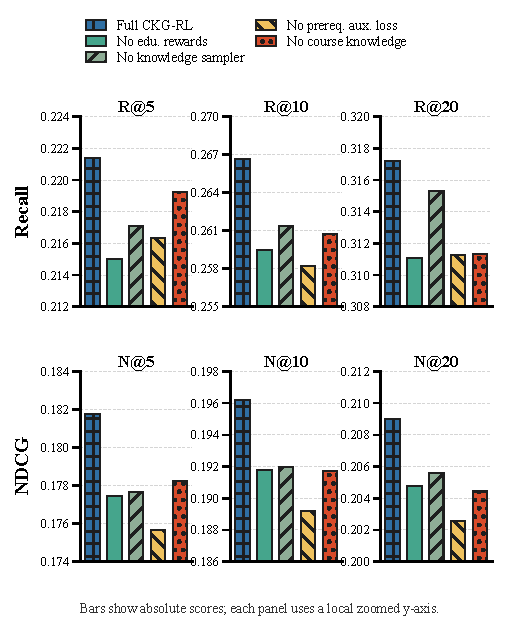
\includegraphics[width=\columnwidth]{figures/mooccube_complete_ablation_core_reference_style_single_column.pdf}
\caption{Single-column component ablation bar chart on MOOCCube under strict item-cold full-ranking evaluation. Each local-axis panel reports an absolute item-macro score for Full CKG-RL and variants that remove educational rewards, the knowledge-guided sampler, the prerequisite auxiliary loss, or all course-knowledge inputs.}
\Description{Six grouped bar-chart panels show Recall and NDCG scores at cutoffs 5, 10, and 20 with local zoomed y-axes. Color and hatch encodings distinguish Full CKG-RL, No educational rewards, No knowledge-guided sampler, No prerequisite auxiliary loss, and No course-knowledge inputs.}
\label{fig:ablation-main}
\end{figure}

\subsection{RQ3: Course-Knowledge Ablation}
Figure~\ref{fig:ablation-main} evaluates core-component ablations on MOOCCube under the same split, candidate set, \(K\) values, and item-macro aggregation as Table~\ref{tab:mooccube-cold}. Each variant removes one major part of the CKG-RL design: educational rewards, the knowledge-guided sampler, the prerequisite auxiliary loss, or all course-knowledge inputs.

The core ablations show that the MOOCCube gain is distributed across the major CKG-RL components. Removing educational rewards reduces R@10 by 0.0072 and N@10 by 0.0044, and removing the knowledge-guided sampler reduces R@10 by 0.0053 and N@10 by 0.0043. The prerequisite auxiliary loss gives the largest early-rank NDCG drop among the core ablations, decreasing N@5 by 0.0061 and N@10 by 0.0070, which is consistent with its role in discouraging prerequisite-unsafe matches.

Removing all course-knowledge inputs is also weaker than Full CKG-RL across all six metrics. The result supports a bounded conclusion: the MOOCCube improvement relies on course knowledge when it is coupled to educational rewards, candidate construction, and auxiliary supervision, rather than on a single scalar signal alone.

\FloatBarrier

\subsection{RQ4: Hyperparameter Sensitivity}
We evaluate the MOOCCube main-table configuration under three hyperparameter sweeps: knowledge-sampling weight \(\beta\), reward-shaping scale, and simulator horizon \(T\). Each point is averaged over the same three seeds used in the main tables. The sweep is intended as a sensitivity analysis rather than a separate tuning protocol: it tests whether the reported configuration lies in a stable region of the design space.

\begin{figure}[t]
\centering
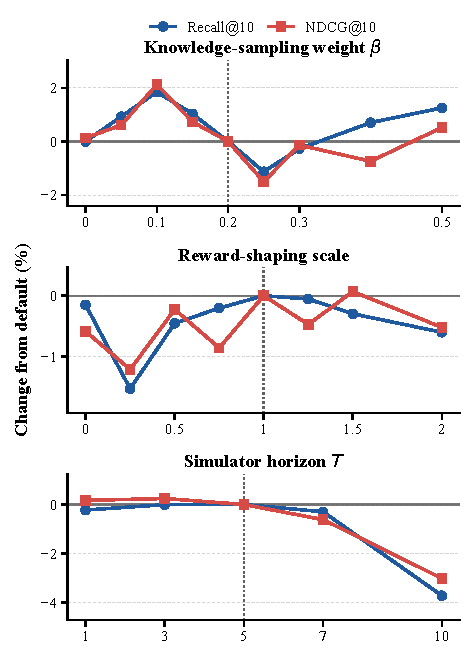
\includegraphics[width=\columnwidth]{figures/mooccube_hparam_sensitivity_single_column.pdf}
\caption{Single-column MOOCCube hyperparameter sensitivity for knowledge-sampling weight \(\beta\), reward-shaping scale, and simulator horizon \(T\). The y-axis reports percentage change from the default score, and dotted lines mark default values.}
\Description{Three line charts show relative Recall at 10 and NDCG at 10 changes for sweeps over knowledge-sampling weight, reward-shaping scale, and simulator horizon. Scores vary within a narrow band around the default, while horizon 10 drops more noticeably.}
\label{fig:hparam-sensitivity}
\end{figure}

Figure~\ref{fig:hparam-sensitivity} shows bounded variation around the default setting. For the knowledge-sampling weight \(\beta\), R@10 spans 0.2636 to 0.2716 and N@10 spans 0.1933 to 0.2004, with no monotonic preference for larger knowledge-sampling weight. Reward-shaping scale stays in a narrow band around the default scale \(1.0\), which gives 0.2667 R@10 and 0.1962 N@10. Simulator horizons \(T=1,3,5,7\) perform similarly, whereas \(T=10\) drops to 0.2568 R@10 and 0.1903 N@10. Thus, the MOOCCube result does not depend on a single sharp hyperparameter optimum; moderate horizons are stable, while excessive rollout length can dilute the target-course signal.

\subsection{RQ5: Computational Cost}
Table~\ref{tab:runtime} reports the timing evidence that can be separated from the current main-experiment logs. The CKG-RL training logs print a training-loop time before validation ranking, so the reported values are average seconds per training epoch and exclude validation and test evaluation. The COCO CGRC logs also expose complete per-epoch progress timers, allowing a direct training-loop comparison on that dataset. Other baseline logs in the main tables report metrics and, in some queue files, end-to-end process wall-clock time, but they do not separately log one training epoch or final full-ranking inference time. We therefore do not convert those mixed wall-clock records into per-epoch or inference numbers.

\begin{table*}[t]
\centering
\caption{Logged training-loop timing for methods whose main-experiment logs expose separable epoch timers. Values are mean \(\pm\) standard deviation in seconds. Isolated full-ranking inference timers were not emitted by the current logs.}
\label{tab:runtime}
\small
\setlength{\tabcolsep}{4.0pt}
\renewcommand{\arraystretch}{1.08}
\begin{tabular}{llccp{5.2cm}}
\toprule
Dataset & Method & Train epoch (s) & Inference timer & Logged coverage \\
\midrule
MOOCCube & CKG-RL & \(133.8\pm51.8\) & not logged separately & 3 seeds, 180 training epochs. \\
Junyi & CKG-RL & \(312.2\pm67.4\) & not logged separately & 2 logged seeds, 120 training epochs. \\
COCO & CKG-RL & \(279.2\pm17.7\) & not logged separately & 3 seeds, 90 training epochs. \\
COCO & CGRC~\cite{kim2024cgrc} & \(389.7\pm79.7\) & not logged separately & 3 seeds, 150 training epochs. \\
\bottomrule
\end{tabular}
\end{table*}

These measurements support a bounded efficiency conclusion. CKG-RL is more expensive per training example than simple collaborative or content baselines in Table~\ref{tab:complexity}, because the simulator retrieves \(M=256\) users and samples \(N=20\) candidates across \(T=5\) steps. However, the overhead is not catalog-wide during training, and on COCO the logged CKG-RL epoch time is lower than the logged CGRC epoch time. At inference time, CKG-RL does not roll out the simulator for every candidate in the full catalog; it builds item vectors and then uses the same catalog dot-product scoring pattern as the embedding baselines. The current implementation should therefore be read as training-heavier than simple baselines, but not as changing the asymptotic full-ranking inference bottleneck.

\section{Discussion}
\subsection{Why Item-Macro Matters}
The strict item-cold setting changes the meaning of progress. A method can improve interaction-weighted metrics by performing well on a few cold courses with many test interactions, while still leaving other cold courses without useful ranks. Item-macro aggregation makes this failure visible by assigning each cold course equal weight. In this sense, the metric acts as a risk-sensitive diagnostic. It penalizes systems that achieve acceptable average performance while neglecting individual item-cold courses. This is why the main claim is based on item-macro full-ranking scores rather than sampled ranking or aggregate user-level metrics.

\subsection{Cold-Hot Trade-Off}
Course knowledge plays complementary roles across recommendation regimes. Concept overlap provides a semantic bridge under sparse evidence, while prerequisite and difficulty signals add readiness-oriented structure when learner histories provide enough context. The cold-hot profile should therefore be read as a design signal: CKG-RL uses the same course-knowledge inputs to strengthen item-cold exposure, and the relative contribution of each input can be further adapted to the amount of learner history available.

\subsection{Implications for Item-Cold Exposure}
The strict item-cold protocol approximates one important part of course introduction: ranking an item when its own interactions are unavailable. At this stage, the system cannot wait for collaborative signals on the target course to mature. It must use course-side evidence to identify plausible early audiences. Item-macro full-ranking evaluation makes this exposure problem visible by asking whether many item-cold courses receive useful ranks, not only whether the most frequently clicked cold courses do well. This diagnostic can complement chronological launch evaluation by isolating the representation problem before exposure feedback begins.

\section{Limitations}
The strict item-cold evaluation contains about 68 cold courses per seed on MOOCCube, 71 cold items per seed on Junyi, and 820 cold items per seed on COCO. These are meaningful controlled benchmarks but remain limited relative to industrial catalogs. Larger catalogs may include more heterogeneous course descriptions, provider incentives, and exposure constraints. Additional datasets and cold-ratio sensitivity studies would strengthen external validity.

The course relations and content embeddings are dataset-specific, and the quality of prerequisites or concept mappings can affect reward reliability. The prerequisite and difficulty signals are approximations of learning readiness, not direct measurements of mastery. Difficulty is estimated from inverse popularity, and readiness is estimated from observed history length. In settings with noisy concept graphs, incomplete prerequisite annotations, or weak content embeddings, the same reward terms may need confidence weighting or human validation.

Finally, this paper focuses on offline ranking accuracy. Full-ranking item-macro metrics make item-cold exposure risk visible, but they do not measure downstream learning outcomes, learner satisfaction, or long-term educational impact. A deployment study would need to test whether improved cold-course ranking leads to beneficial learning behavior rather than only more exposure for item-cold courses.

\section{Conclusion}
We studied MOOC recommendation under a strict item-cold protocol that isolates courses with no training interactions. Full-ranking item-macro evaluation exposes a risk that interaction averages can hide: individual item-cold courses may receive no useful exposure even when average performance appears acceptable. CKG-RL addresses this condition with content-anchored representations, forced-cold ID masking, retrieval-based simulation, and course-knowledge rewards. Across MOOCCube, Junyi, and COCO, it improves the primary early-rank item-cold metrics over strong baselines under matched full-ranking evaluation. The results support a protocol-aware view of cold-start recommendation: reducing item-cold exposure risk requires both content transfer and educational constraints, and its benefits should be interpreted within the offline ranking boundary studied here.

\section{Ethical Considerations}
The experiments use public MOOCCube/MOOCCubeX, Junyi, and COCO educational interaction data and derived item representations. Because such logs may reflect sensitive learner behavior, released artifacts should avoid personally identifiable information and follow dataset access conditions. The method is evaluated offline and should not be treated as evidence of improved learner outcomes without online or pedagogical validation. In deployment, course recommenders may affect attention, course visibility, and educational opportunity; operators should monitor fairness, provide appropriate transparency, and avoid using recommendations as the sole basis for consequential educational decisions.

\bibliographystyle{ACM-Reference-Format}
\bibliography{references}

\end{document}
